\documentclass[english,a4paper,twoside]{ppfcmthesis}

\usepackage[utf8]{inputenc}
\usepackage[OT4]{fontenc}
\usepackage{tabularx}
\usepackage{listings}
\usepackage{enumitem}
\usepackage{lmodern}
\usepackage{booktabs}
\usepackage{float}
\usepackage{placeins}
\usepackage{colortbl}
\usepackage{siunitx}
\usepackage{subcaption}
\usepackage{array}
\usepackage{pgfplotstable}
\usepackage{csvsimple}
\usepackage{hyperref}
\usepackage[algoruled]{algorithm2e}
\usepackage{amsmath}
\usepackage{amsthm}
\usepackage{pdfpages}
\usepackage{xifthen}

% DRAFT
% \usepackage{draftwatermark}
% \SetWatermarkLightness{0.9}
% END DRAFT

\DeclareGraphicsExtensions{.pdf,.png,.jpg}
% \usepackage{tikz}
% \usetikzlibrary{arrows}
\usepackage{ifthen}

\author{
   Amadeusz Juskowiak \album{106453} \and
   Wioletta Różańska \album{xxxxxx}}

\title{Road to solving quadratic assignment problem using Physarum Machines}

\ppsupervisor{Professor~Jacek~Błażewicz}
\ppyear{2016}

\newlength\longest

\lstset{
  basicstyle=\ttfamily\footnotesize, 
  basewidth={0.5em,0.5em}, 
  frame=single, 
  breaklines=true, 
  language=C++
}

\graphicspath{ {figures/} }

%algorithm2e
\SetAlgorithmName{Pseudocode}{List of pseudocodes}

\begin{document}
\graphicspath{{figures/}}
% Front matter starts here
\frontmatter\pagestyle{empty}%
\maketitle\cleardoublepage%

% 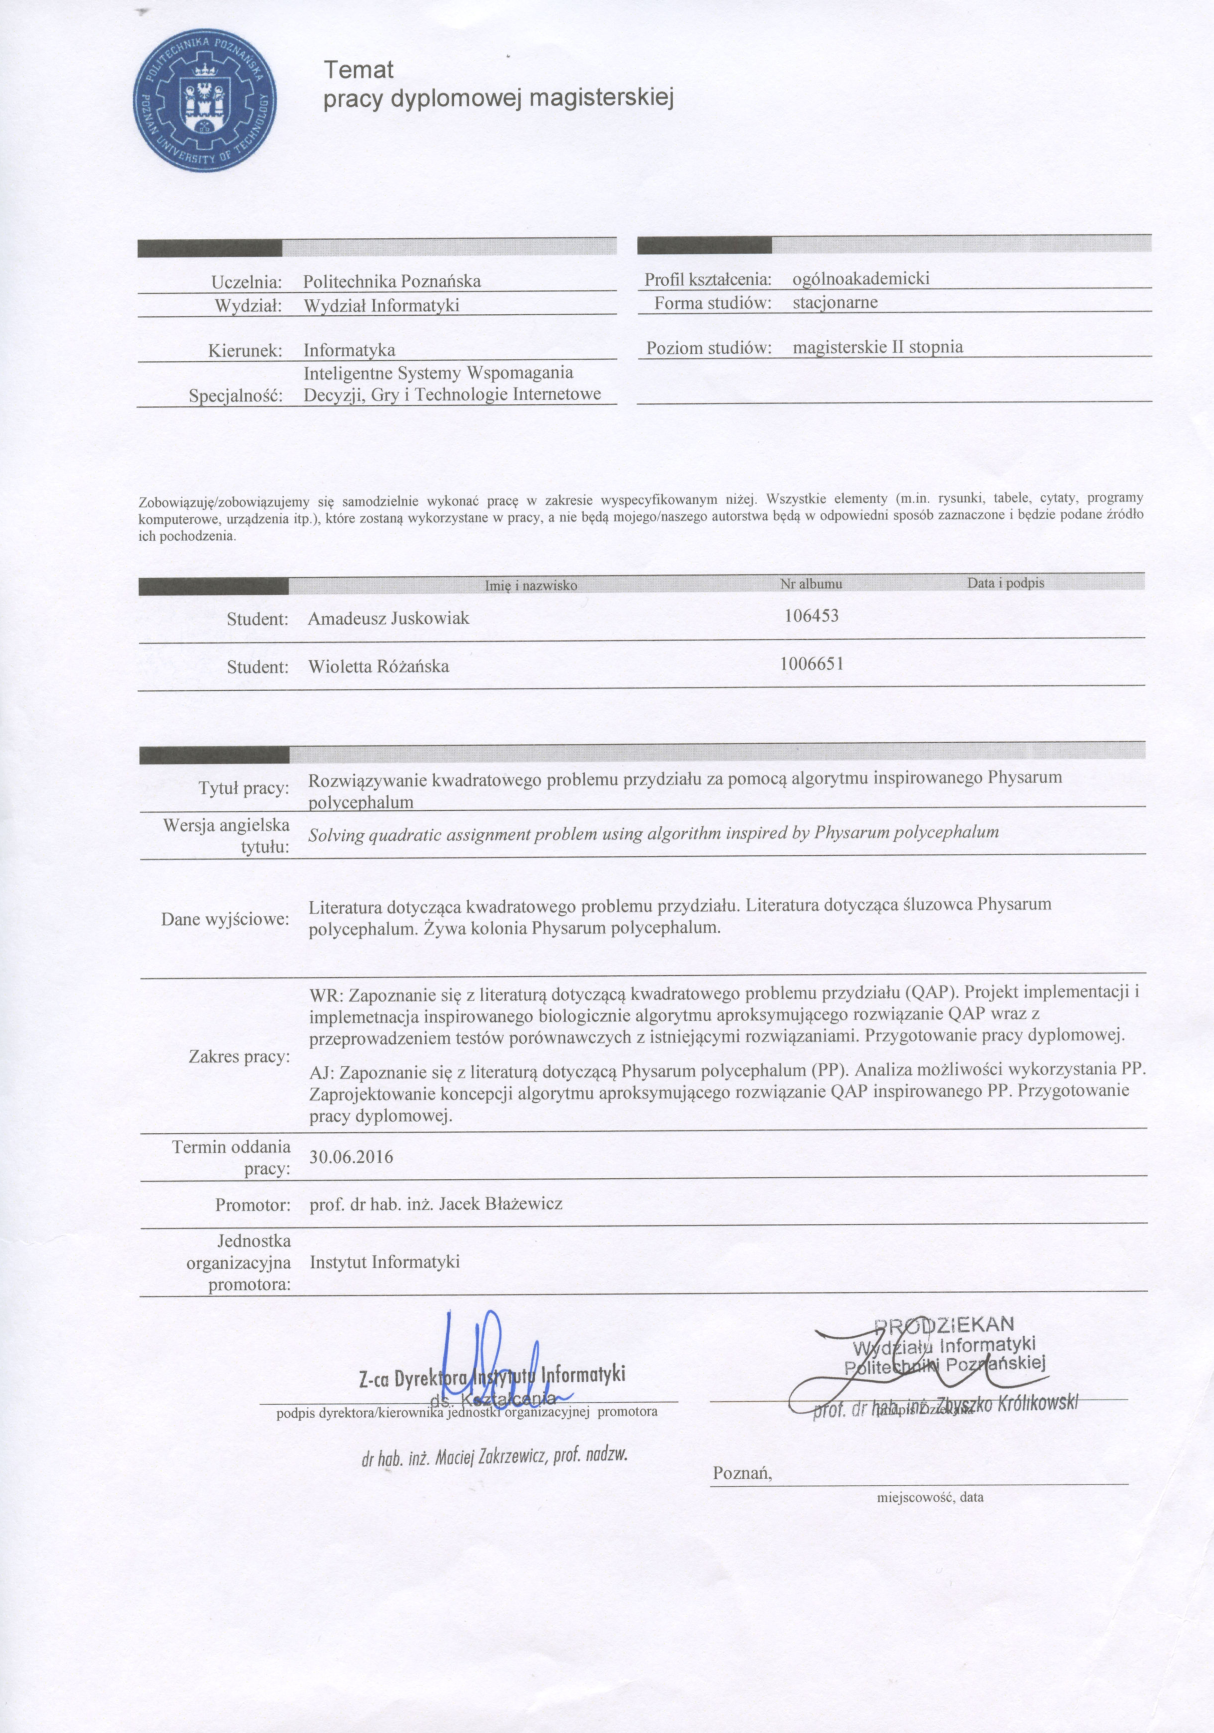
\includepdf{figures/karta.pdf}
% \cleardoublepage

\pagenumbering{gobble}

% \chapter*{Acknowledgements}

{
\null\vfill\hfill
\settowidth\longest{\itshape His work is like that of the planter --- for the future. bla bla bla}
\centering
\parbox{\longest}{%
  \raggedright{\itshape%
  The scientific man does not aim
  at an immediate result. He does not
  expect that his advanced ideas
  will be readily taken up. \\
  \vspace{\baselineskip}
  His work is like that of the planter --- for the future. \\ 
  His duty is to lay the foundation for those who are to come, and point the way.\par\bigskip
  }   
  \raggedleft\MakeUppercase{Nikola Tesla}\par%
}
}

% \cleardoublepage
% \chapter*{Abstract}

The Quadratic Assignment Problem is an optimisation problem with many practical usecases, even though its solutions are usually approximated. It is a representant of NP-hard computation class, therefore there is no algorithm known for solving this problem in polynomial time. Even for a small instances, the computation of the exact assignment can take too much time, which makes it unpractical. This creates a need for various heuristical methods for approximating the solution, which can be used in fields of logistics, computer aided design or even molecular chemistry.

Recently, an emerging computational behaviour of \textit{Physarum polycephalum} is a subject for thorough research. Many works already describe this slime mould as useful in various branches of the computing science. The plasmodial form of \textit{Physarum polycephalum} is used to solve a maze problem, provide a design for a robust network or even approximate the Travelling Salesman Problem. The slime mould is even mathematically modelled and simulated on various levels.

In context of these observations, we transform the gained knowledge of both fields of QAP and \textit{Physarum polycephalum} into an algorithm leading to an approximation of Quadratic Assignment Problem. By observations of a living plasmodium, some of its behaviour is used in a design of the Physarum-based Metaheuristic. This novel method of looking through the search space is used to solve QAP.

As a part of this thesis an implementation of the proposed algorithm is given.After thorough tests, it provides an useful solutions for many practical usecases. Furthermore it can be tuned to solve a complex instances of QAP or even used for approximating other optimisation problems.

% \cleardoublepage

% Table of contents.
\pagenumbering{Roman}\pagestyle{ppfcmthesis}%
\tableofcontents* \cleardoublepage%

% Main content of your thesis starts here.
\mainmatter%
% \chapter{Introduction}
\label{chapter:introduction}

Nowadays, computing science intertwines with various fields of studies posing new challenges for the people of the industry. Every aspect of science is dominated by the technology, just like the everyday lives across the world.

A good example of such interdisciplinary connection is a situation when the companies' managers are required to answer a difficult optimisation question. These businesses mostly are made of different branches, which require transferring of goods between them. Each element of the product could be manufactured in a various departments and is needed in the last part of the assembly in the main office. It could be easier when they produce the whole product in one location, yet seldom it is better to divide the responsibility for specialists in each sector. Although, this process generates som extra costs for the company, it would be crucial to minimise the expenses during assignment of the branches to the locations. Trying to resolve this by hand could be a long process due to the complexity of the problem. However, with usage of computers, it could be answered in a shorter time. The result may not be the optimal one in each case, but it should meet most given assumptions, which is enough to put it into real life usage.

In computer science, this dilemma can be stated as the Quadratic Assignment Problem (QAP).  The QAP is a combinatorial optimisation problem, which was defined by Koopmans and Beckmann in 1957 \cite{koopmans-beckmann1957}, and is a generalisation of an assignment problem. It is NP-hard thus even for small instances finding results is done by approximate methods.

The QAP can be formulated as follows: Given $ n $ different facilities ($F$) and $ n $ different locations ($L$), a weight function $ w: F \times F \mapsto R $ between facilities and a distance function $ d: L \times L \mapsto R $ between locations, find the assignment minimising this cost function:

\begin{equation}
min \sum_{a, b \in P } w(a, b) * d( f(a), f(b))
\end{equation}

Over the years, a number of methods for solving this problem were established. Nevertheless, there is still a place for improvement and experts are searching for new ways of resolving that. Inspired by their works this thesis tries to find an innovative method using living organisms.

The \textit{Physarum Polycephalum}, also known as a true slime mould, is a plasmodial organism of yellow colour. Its single cell body is considered to be the biggest in the world \cite{stephenson1994myxomycetes}. Taking into account current state of classification, it belongs to the Kingdom Protista, however, this used to frequently change due to the fact that it does not exactly match any of the recognised kingdoms. The organisms move very slowly, in a branching pattern as it forages for new food sources. It ingests bacteria, fungal spores and during the experiments --- oatmeals.

\section{Motivation}
\label{section:introduction_motivation}

The motivation for this thesis was indirect interest in topics related to computer science, but also of the world around us. The behavior of physarum, which is often compared to a simple machine, creates many opportunities to unveil a biological side of computer science making the topic fascinating.

Nowadays, scientists put great emphasis on discovering and analyzing the nature. It is done to improve the world surrounding us. Generally, two ways of development of this field of study could be distinguished. The first one focuses on improving the biological flaws of humans and animals. A good case is studies related to the creation of natural prosthetics that make life easier for the people without limbs. The second one is a transmission of the known naturally patterns to the computing environment. Observing the nature leads to logical algorithms, which usage can solve issues seemingly unrelated to originally presented problems and often gives much better solution than working it out greedy. For example, thanks to such research, the ant algorithm was implemented, which shows the behavior of an ant colony searching for the best path between their home and food. These unconventional methods of inventing algorithms allow excellent results for hitherto very complicated mathematical problems.

The physarums have great potential in both, the first and the second case. Until now, several studies linked to these organisms were conducted, though, it still remains a mystery to many experts. One example of an experiment carried on slime molds was solving the maze. The organism found the shortest path between two oatmeals in the environment with walls, thus finding the solution for the maze. More detailed description and more cases are presented in the later chapter of this thesis. Nonetheless, these interesting achievements were the reason behind the choice of the subject.

Also, the thesis focuses on the quadratic assignment problem, which is a challenging topic. It reflects the real difficulties faced by the managers of logistics companies. They need optimal results, however, the complexity of the dilemma makes it almost impossible to resolve in a reasonable time. This demand urges scientists to explore this issue further and try to look for a reliable way of solving the problem. 

The QAP could be a great challenge for inventing a new unconventional algorithm based on the behavior of physarum. 

\section{Goal}
\label{section:introduction_goal}

This thesis presents the road to solving Quadratic Assignment Problem (QAP) based on behaviour of physarum machines. In order to reach meaningful conclusions, it is needed to analyse deeply each part of the main dilemma.

The first task is carrying out the detailed investigation of the behaviour and capabilities of the slime mould. Without the understanding of organisms, it is not possible to replicate its operations. For this purpose, the living plasmodia will be observed, giving us details of the schemes how it moves when looking for food. This will be studied in order to extract similar patterns and facilitate the creation of their calculation method, which could be transported into the computer environment. We will implement such plasmodial behaviour for solving QAP.

Furthermore, not only the direct observation of their behavior is needed here, but also a careful examination of previous studies. Such research will give as a thorough look into behaviour and abilities of the slime mould.

Next, the analysis of the research related to the QAP will be conducted, leading to better understanding of the problem and showing the current practices for solving it. Recognising the dilemma will make it easier to fit algorithm based on slime moulds to the QAP.

The key element of this thesis is applying physarum methods for solving QAP. This step will consist of adapting the mechanisms, implementation of simulation and reading its results. It will summarise the previously acquired theoretical knowledge in a practical task.

And last, but not least, our aim will be to create the innovative method for solving QAP.


\section{Chapters}
\label{section:introduction_chapters}

The thesis is divided into five chapters and includes three appendices.

\begin{itemize}
  \item Chapter 2 describes the research conducted in order to better understand the problems. It is divided into two parts. The first one describes the physarum organisms characteristics such as a position in the hierarchy, basic information about the species, basics of operations, emerging behaviour and previous research. The second outlines the quadratic assignment problem (QAP). It consists of a different interpretation, practical usages, current exact solution and current heuristic.
  \item Chapter 3 presents an idea for a physarum machine and an algorithm, being a main matter for this thesis. It will be a pseudophysarum machine providing working metaheuristics based on observed behavior.
  \item Chapter 4 describes an implementation of the algorithm and thorougly tests its behaviour and capabilities.
  \item Chapter 5 summarises our research and gives ideas for future work.
  \item Appendix A includes methods of working with a living colony of \textit{Physarum Polycephalum}.
  \item Appendix B provides detailed results in tabular form.
  \item Appendix C extends the work with usage of the algorithm for simplified tests for related Travelling Salesman Problem.
\end{itemize}


\section*{Work Distribution}
\label{section:introduction_distribution}

Both authors wrote the text of this thesis. The rest of the work was distributed between two co-workers in a manner described below:
\begin{itemize}
  \item Amadeusz Juskowiak conducted a research about \textit{Physarum polycephalum} and observed the behaviour of the alive organisms. He also designed and implemented the algorithm approximating QAP.
  \item Wioletta Różańska conducted a research about the quadratic assignment problem. She also implemented the algorithm approximating QAP and carried out comparative tests with existing solutions.
\end{itemize}



% \cleardoublepage\appendix
% \input{"chapters/appendices/test_results.tex"}

% Bibliography (books, articles) starts here.
\bibliographystyle{alpha}{\raggedright\sloppy\small\bibliography{bibliography}}

% Colophon is a place where you should let others know about copyrights etc.
\cleardoublepage\ppcolophon

\end{document}
